% Created by tikzDevice version 0.10.1 on 2016-09-01 14:03:52
% !TEX encoding = UTF-8 Unicode
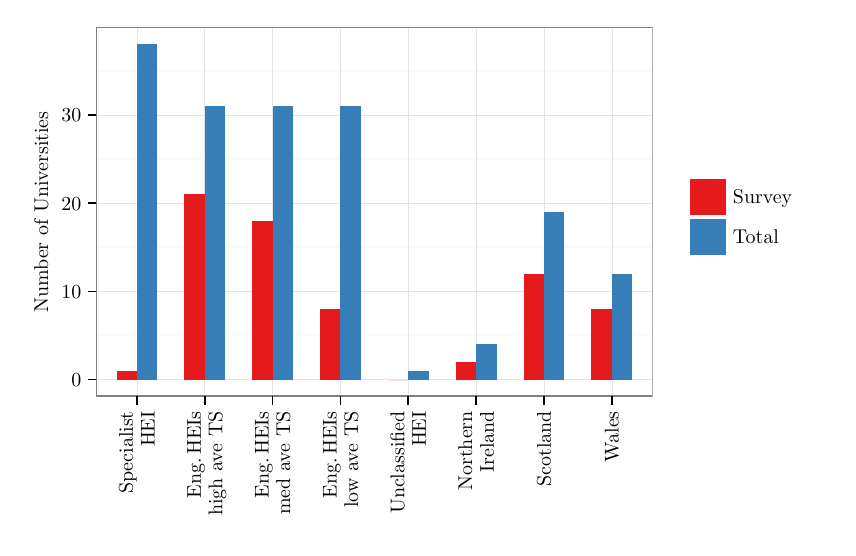
\begin{tikzpicture}[x=1pt,y=1pt]
\definecolor{fillColor}{RGB}{255,255,255}
\path[use as bounding box,fill=fillColor,fill opacity=0.00] (0,0) rectangle (289.08,180.67);
\begin{scope}
\path[clip] (  0.00,  0.00) rectangle (289.08,180.67);
\definecolor{drawColor}{RGB}{255,255,255}
\definecolor{fillColor}{RGB}{255,255,255}

\path[draw=drawColor,line width= 0.6pt,line join=round,line cap=round,fill=fillColor] (  0.00,  0.00) rectangle (289.08,180.68);
\end{scope}
\begin{scope}
\path[clip] ( 24.76, 47.46) rectangle (225.80,180.67);
\definecolor{fillColor}{RGB}{255,255,255}

\path[fill=fillColor] ( 24.76, 47.46) rectangle (225.80,180.67);
\definecolor{drawColor}{gray}{0.98}

\path[draw=drawColor,line width= 0.6pt,line join=round] ( 24.76, 69.45) --
	(225.80, 69.45);

\path[draw=drawColor,line width= 0.6pt,line join=round] ( 24.76,101.32) --
	(225.80,101.32);

\path[draw=drawColor,line width= 0.6pt,line join=round] ( 24.76,133.19) --
	(225.80,133.19);

\path[draw=drawColor,line width= 0.6pt,line join=round] ( 24.76,165.06) --
	(225.80,165.06);
\definecolor{drawColor}{gray}{0.90}

\path[draw=drawColor,line width= 0.2pt,line join=round] ( 24.76, 53.51) --
	(225.80, 53.51);

\path[draw=drawColor,line width= 0.2pt,line join=round] ( 24.76, 85.38) --
	(225.80, 85.38);

\path[draw=drawColor,line width= 0.2pt,line join=round] ( 24.76,117.25) --
	(225.80,117.25);

\path[draw=drawColor,line width= 0.2pt,line join=round] ( 24.76,149.12) --
	(225.80,149.12);

\path[draw=drawColor,line width= 0.2pt,line join=round] ( 39.47, 47.46) --
	( 39.47,180.67);

\path[draw=drawColor,line width= 0.2pt,line join=round] ( 63.98, 47.46) --
	( 63.98,180.67);

\path[draw=drawColor,line width= 0.2pt,line join=round] ( 88.50, 47.46) --
	( 88.50,180.67);

\path[draw=drawColor,line width= 0.2pt,line join=round] (113.02, 47.46) --
	(113.02,180.67);

\path[draw=drawColor,line width= 0.2pt,line join=round] (137.54, 47.46) --
	(137.54,180.67);

\path[draw=drawColor,line width= 0.2pt,line join=round] (162.05, 47.46) --
	(162.05,180.67);

\path[draw=drawColor,line width= 0.2pt,line join=round] (186.57, 47.46) --
	(186.57,180.67);

\path[draw=drawColor,line width= 0.2pt,line join=round] (211.09, 47.46) --
	(211.09,180.67);
\definecolor{fillColor}{RGB}{228,26,28}

\path[fill=fillColor] ( 32.11, 53.51) rectangle ( 39.47, 56.70);
\definecolor{fillColor}{RGB}{55,126,184}

\path[fill=fillColor] ( 39.47, 53.51) rectangle ( 46.82,174.62);
\definecolor{fillColor}{RGB}{228,26,28}

\path[fill=fillColor] ( 56.63, 53.51) rectangle ( 63.98,120.44);
\definecolor{fillColor}{RGB}{55,126,184}

\path[fill=fillColor] ( 63.98, 53.51) rectangle ( 71.34,152.31);
\definecolor{fillColor}{RGB}{228,26,28}

\path[fill=fillColor] ( 81.15, 53.51) rectangle ( 88.50,110.88);
\definecolor{fillColor}{RGB}{55,126,184}

\path[fill=fillColor] ( 88.50, 53.51) rectangle ( 95.86,152.31);
\definecolor{fillColor}{RGB}{228,26,28}

\path[fill=fillColor] (105.66, 53.51) rectangle (113.02, 79.01);
\definecolor{fillColor}{RGB}{55,126,184}

\path[fill=fillColor] (113.02, 53.51) rectangle (120.37,152.31);
\definecolor{fillColor}{RGB}{228,26,28}

\path[fill=fillColor] (130.18, 53.51) rectangle (137.54, 53.51);
\definecolor{fillColor}{RGB}{55,126,184}

\path[fill=fillColor] (137.54, 53.51) rectangle (144.89, 56.70);
\definecolor{fillColor}{RGB}{228,26,28}

\path[fill=fillColor] (154.70, 53.51) rectangle (162.05, 59.89);
\definecolor{fillColor}{RGB}{55,126,184}

\path[fill=fillColor] (162.05, 53.51) rectangle (169.41, 66.26);
\definecolor{fillColor}{RGB}{228,26,28}

\path[fill=fillColor] (179.21, 53.51) rectangle (186.57, 91.76);
\definecolor{fillColor}{RGB}{55,126,184}

\path[fill=fillColor] (186.57, 53.51) rectangle (193.92,114.07);
\definecolor{fillColor}{RGB}{228,26,28}

\path[fill=fillColor] (203.73, 53.51) rectangle (211.09, 79.01);
\definecolor{fillColor}{RGB}{55,126,184}

\path[fill=fillColor] (211.09, 53.51) rectangle (218.44, 91.76);
\definecolor{drawColor}{gray}{0.50}

\path[draw=drawColor,line width= 0.6pt,line join=round,line cap=round] ( 24.76, 47.46) rectangle (225.80,180.67);
\end{scope}
\begin{scope}
\path[clip] (  0.00,  0.00) rectangle (289.08,180.67);
\definecolor{drawColor}{RGB}{0,0,0}

\node[text=drawColor,anchor=base east,inner sep=0pt, outer sep=0pt, scale=  0.72] at ( 19.36, 51.03) {0};

\node[text=drawColor,anchor=base east,inner sep=0pt, outer sep=0pt, scale=  0.72] at ( 19.36, 82.90) {10};

\node[text=drawColor,anchor=base east,inner sep=0pt, outer sep=0pt, scale=  0.72] at ( 19.36,114.77) {20};

\node[text=drawColor,anchor=base east,inner sep=0pt, outer sep=0pt, scale=  0.72] at ( 19.36,146.64) {30};
\end{scope}
\begin{scope}
\path[clip] (  0.00,  0.00) rectangle (289.08,180.67);
\definecolor{drawColor}{RGB}{0,0,0}

\path[draw=drawColor,line width= 0.6pt,line join=round] ( 21.76, 53.51) --
	( 24.76, 53.51);

\path[draw=drawColor,line width= 0.6pt,line join=round] ( 21.76, 85.38) --
	( 24.76, 85.38);

\path[draw=drawColor,line width= 0.6pt,line join=round] ( 21.76,117.25) --
	( 24.76,117.25);

\path[draw=drawColor,line width= 0.6pt,line join=round] ( 21.76,149.12) --
	( 24.76,149.12);
\end{scope}
\begin{scope}
\path[clip] (  0.00,  0.00) rectangle (289.08,180.67);
\definecolor{drawColor}{RGB}{0,0,0}

\path[draw=drawColor,line width= 0.6pt,line join=round] ( 39.47, 44.46) --
	( 39.47, 47.46);

\path[draw=drawColor,line width= 0.6pt,line join=round] ( 63.98, 44.46) --
	( 63.98, 47.46);

\path[draw=drawColor,line width= 0.6pt,line join=round] ( 88.50, 44.46) --
	( 88.50, 47.46);

\path[draw=drawColor,line width= 0.6pt,line join=round] (113.02, 44.46) --
	(113.02, 47.46);

\path[draw=drawColor,line width= 0.6pt,line join=round] (137.54, 44.46) --
	(137.54, 47.46);

\path[draw=drawColor,line width= 0.6pt,line join=round] (162.05, 44.46) --
	(162.05, 47.46);

\path[draw=drawColor,line width= 0.6pt,line join=round] (186.57, 44.46) --
	(186.57, 47.46);

\path[draw=drawColor,line width= 0.6pt,line join=round] (211.09, 44.46) --
	(211.09, 47.46);
\end{scope}
\begin{scope}
\path[clip] (  0.00,  0.00) rectangle (289.08,180.67);
\definecolor{drawColor}{RGB}{0,0,0}

\node[text=drawColor,rotate= 90.00,anchor=base east,inner sep=0pt, outer sep=0pt, scale=  0.72] at ( 38.06, 42.06) {Specialist};

\node[text=drawColor,rotate= 90.00,anchor=base east,inner sep=0pt, outer sep=0pt, scale=  0.72] at ( 45.83, 42.06) {HEI};

\node[text=drawColor,rotate= 90.00,anchor=base east,inner sep=0pt, outer sep=0pt, scale=  0.72] at ( 62.58, 42.06) {Eng.\,HEIs};

\node[text=drawColor,rotate= 90.00,anchor=base east,inner sep=0pt, outer sep=0pt, scale=  0.72] at ( 70.35, 42.06) {high ave TS};

\node[text=drawColor,rotate= 90.00,anchor=base east,inner sep=0pt, outer sep=0pt, scale=  0.72] at ( 87.09, 42.06) {Eng.\,HEIs};

\node[text=drawColor,rotate= 90.00,anchor=base east,inner sep=0pt, outer sep=0pt, scale=  0.72] at ( 94.87, 42.06) {med ave TS};

\node[text=drawColor,rotate= 90.00,anchor=base east,inner sep=0pt, outer sep=0pt, scale=  0.72] at (111.61, 42.06) {Eng.\,HEIs};

\node[text=drawColor,rotate= 90.00,anchor=base east,inner sep=0pt, outer sep=0pt, scale=  0.72] at (119.39, 42.06) {low ave TS};

\node[text=drawColor,rotate= 90.00,anchor=base east,inner sep=0pt, outer sep=0pt, scale=  0.72] at (136.13, 42.06) {Unclassified};

\node[text=drawColor,rotate= 90.00,anchor=base east,inner sep=0pt, outer sep=0pt, scale=  0.72] at (143.90, 42.06) {HEI};

\node[text=drawColor,rotate= 90.00,anchor=base east,inner sep=0pt, outer sep=0pt, scale=  0.72] at (160.64, 42.06) {Northern};

\node[text=drawColor,rotate= 90.00,anchor=base east,inner sep=0pt, outer sep=0pt, scale=  0.72] at (168.42, 42.06) {Ireland};

\node[text=drawColor,rotate= 90.00,anchor=base east,inner sep=0pt, outer sep=0pt, scale=  0.72] at (189.05, 42.06) {Scotland};

\node[text=drawColor,rotate= 90.00,anchor=base east,inner sep=0pt, outer sep=0pt, scale=  0.72] at (213.57, 42.06) {Wales};
\end{scope}
\begin{scope}
\path[clip] (  0.00,  0.00) rectangle (289.08,180.67);
\definecolor{drawColor}{RGB}{0,0,0}

\node[text=drawColor,rotate= 90.00,anchor=base,inner sep=0pt, outer sep=0pt, scale=  0.72] at (  7.36,114.07) {Number of Universities};
\end{scope}
\begin{scope}
\path[clip] (  0.00,  0.00) rectangle (289.08,180.67);
\definecolor{fillColor}{RGB}{255,255,255}

\path[fill=fillColor] (234.33, 93.54) rectangle (280.54,134.60);
\end{scope}
\begin{scope}
\path[clip] (  0.00,  0.00) rectangle (289.08,180.67);
\definecolor{fillColor}{RGB}{228,26,28}

\path[fill=fillColor] (239.31,112.97) rectangle (252.34,126.00);
\end{scope}
\begin{scope}
\path[clip] (  0.00,  0.00) rectangle (289.08,180.67);
\definecolor{fillColor}{RGB}{55,126,184}

\path[fill=fillColor] (239.31, 98.52) rectangle (252.34,111.55);
\end{scope}
\begin{scope}
\path[clip] (  0.00,  0.00) rectangle (289.08,180.67);
\definecolor{drawColor}{RGB}{0,0,0}

\node[text=drawColor,anchor=base west,inner sep=0pt, outer sep=0pt, scale=  0.72] at (254.86,117.01) {Survey};
\end{scope}
\begin{scope}
\path[clip] (  0.00,  0.00) rectangle (289.08,180.67);
\definecolor{drawColor}{RGB}{0,0,0}

\node[text=drawColor,anchor=base west,inner sep=0pt, outer sep=0pt, scale=  0.72] at (254.86,102.55) {Total};
\end{scope}
\end{tikzpicture}
